\documentclass[11pt,a4paper]{article}

\usepackage[margin=2.1cm]{geometry}
\usepackage{hyperref}
\usepackage{booktabs}
\usepackage{longtable}
\usepackage{enumitem}
\usepackage{graphicx}
\usepackage{xcolor}
\usepackage{listings}
\usepackage{fancyhdr}
\usepackage{array}
\usepackage{parskip}
\usepackage{tabularx}
\usepackage{tikz}
\usetikzlibrary{arrows.meta,positioning,fit,calc}

\hypersetup{
  colorlinks=true,
  linkcolor=blue!50!black,
  urlcolor=blue!60!black
}

\pagestyle{fancy}
\fancyhf{}
\fancyhead[L]{\small UGV Vision Navigation --- Architecture Overlay}
\fancyhead[R]{\small Teaching Guide}
\fancyfoot[C]{\thepage}
\renewcommand{\headrulewidth}{0.4pt}

\title{\textbf{UGV Vision Navigation}\\[0.35em]
\large Architecture Overlay Document\\[0.15em]
\normalsize Stereo + VIO + Semantic Nav2 --- Flowchart, Contracts \& Plan}
\author{Team Internship / Vision Navigation Stack}
\date{\today}

\lstset{
  basicstyle=\ttfamily\footnotesize,
  breaklines=true,
  frame=single,
  backgroundcolor=\color{gray!8},
  columns=fullflexible
}

\newcommand{\needs}[1]{\textbf{Needs:} #1}
\newcommand{\provides}[1]{\textbf{Provides:} #1}
\newcommand{\feeds}[1]{\textbf{Feeds to:} #1}

\begin{document}
\maketitle

\begin{abstract}
\noindent
This document is the single architecture overlay for the GPS-denied UGV stack.
It contains: (1)~the Stereo + VIO + Semantic Nav2 flowchart,
(2)~glossary of terms,
(3)~for each technology: \emph{what it needs}, \emph{what it provides}, and \emph{who it feeds},
(4)~the implementation plan, (5)~demo commands, and
(6)~SIH 2026 PPT slide fill guide (what SIH asks / what we need / what we will add).
\end{abstract}

\tableofcontents
\newpage

%======================================================================
\section{Problem statement}

\textbf{Goal in one sentence.}
Drive a ground robot from point~A to point~B outdoors \emph{without GPS}, using cameras (and derived depth), understanding the scene, building or using a map, and planning a safe path.

\textbf{Design constraints.}
\begin{itemize}[leftmargin=*]
  \item No GPS (denied / enclosed outdoor courtyard).
  \item Cameras as primary sensing (no lidar required in the core stack).
  \item Simulation first (Gazebo), same architecture transferable to a real robot later.
\end{itemize}

\textbf{Remember in five words:}
\begin{center}
\textbf{Sense $\rightarrow$ Understand $\rightarrow$ Localize/Map $\rightarrow$ Plan $\rightarrow$ Act}
\end{center}

%======================================================================
\section{Architecture flowchart (Stereo + VIO + Semantic Nav2)}

\begin{center}
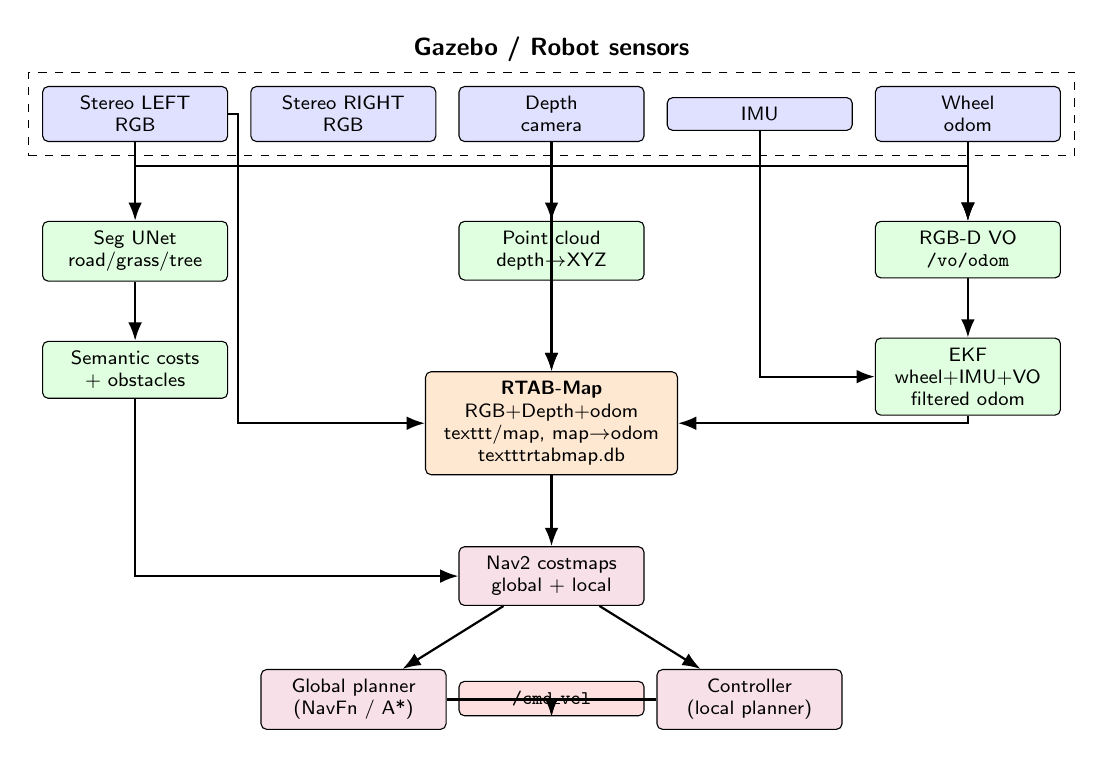
\begin{tikzpicture}[
  font=\sffamily\scriptsize,
  box/.style={draw, rounded corners=2pt, align=center, inner sep=3.5pt, minimum width=2.35cm},
  sensor/.style={box, fill=blue!12},
  proc/.style={box, fill=green!12},
  slam/.style={box, fill=orange!18, minimum width=3.2cm},
  nav/.style={box, fill=purple!12},
  act/.style={box, fill=red!12},
  arrow/.style={-{Latex}, thick},
]
  \node[sensor] (left) {Stereo LEFT\\RGB};
  \node[sensor, right=0.28cm of left] (right) {Stereo RIGHT\\RGB};
  \node[sensor, right=0.28cm of right] (depth) {Depth\\camera};
  \node[sensor, right=0.28cm of depth] (imu) {IMU};
  \node[sensor, right=0.28cm of imu] (wheel) {Wheel\\odom};

  \node[draw, dashed, fit=(left)(right)(depth)(imu)(wheel), inner sep=5pt,
        label={[font=\sffamily\small\bfseries]above:Gazebo / Robot sensors}] {};

  \node[proc, below=1.0cm of left] (unet) {Seg UNet\\road/grass/tree};
  \node[proc, below=1.0cm of depth] (cloud) {Point cloud\\depth$\rightarrow$XYZ};
  \node[proc, below=1.0cm of wheel] (vo) {RGB-D VO\\\texttt{/vo/odom}};
  \node[proc, below=0.75cm of vo] (ekf) {EKF\\wheel+IMU+VO\\filtered odom};

  \draw[arrow] (left) -- (unet);
  \draw[arrow] (depth) -- (cloud);
  \draw[arrow] (left.south) |- ++(0,-0.3) -| (vo.north);
  \draw[arrow] (depth.south) |- ++(0,-0.3) -| (vo.north);
  \draw[arrow] (imu) |- (ekf);
  \draw[arrow] (wheel) -- (vo);
  \draw[arrow] (vo) -- (ekf);

  \node[proc, below=0.75cm of unet] (sem) {Semantic costs\\+ obstacles};

  \draw[arrow] (unet) -- (sem);

  \node[slam, below=1.15cm of cloud] (rtab) {\textbf{RTAB-Map}\\RGB+Depth+odom\\texttt{/map}, map$\rightarrow$odom\\texttt{rtabmap.db}};

  \draw[arrow] (left.east) -- ++(0.12,0) |- (rtab.west);
  \draw[arrow] (depth) -- (rtab);
  \draw[arrow] (ekf) |- (rtab);
  \draw[arrow] (cloud) -- (rtab);

  \node[nav, below=0.9cm of rtab] (cost) {Nav2 costmaps\\global + local};
  \node[nav, below left=0.8cm and 0.15cm of cost] (global) {Global planner\\(NavFn / A*)};
  \node[nav, below right=0.8cm and 0.15cm of cost] (ctrl) {Controller\\(local planner)};
  \node[act, below=0.95cm of cost] (cmd) {\texttt{/cmd\_vel}};

  \draw[arrow] (sem) |- (cost);
  \draw[arrow] (rtab) -- (cost);
  \draw[arrow] (cost) -- (global);
  \draw[arrow] (cost) -- (ctrl);
  \draw[arrow] (global) -| (cmd);
  \draw[arrow] (ctrl) -| (cmd);
\end{tikzpicture}
\end{center}

\noindent\textbf{One-line story.}
Cameras see $\rightarrow$ UNet understands path/hazards $\rightarrow$ EKF+RTAB localize/map $\rightarrow$ Nav2 plans \& controls $\rightarrow$ robot drives A$\rightarrow$B without GPS.

%======================================================================
\section{How to read the ``contracts''}

For every technology below we answer three teaching questions:
\begin{enumerate}[leftmargin=*]
  \item \textbf{Needs (inputs)} --- what must arrive (topics / data / math objects)?
  \item \textbf{Provides (outputs)} --- what does it produce?
  \item \textbf{Feeds to (consumers)} --- who uses that output next?
\end{enumerate}
This is the main learning goal: \emph{who needs what, who provides what, who feeds whom}.

%======================================================================
\section{Module contracts (Needs / Provides / Feeds to)}

%----------------------------------------------------------------------
\subsection{Stereo left RGB camera}
\needs{Light from the scene (physics / Gazebo render).}
\provides{Colour image \texttt{sensor\_msgs/Image} on \texttt{/camera/image\_raw} (alias of left) and \texttt{/stereo/left/image\_raw}; camera info.}
\feeds{Seg UNet; RGB-D visual odometry; RTAB-Map.}

%----------------------------------------------------------------------
\subsection{Stereo right RGB camera}
\needs{Same scene from a second viewpoint (baseline).}
\provides{\texttt{/stereo/right/image\_raw} (+ camera info).}
\feeds{Optional future true stereo disparity; currently not required by RTAB in our sim path.}

%----------------------------------------------------------------------
\subsection{Depth camera}
\needs{Scene geometry in simulation (or a real depth/RGB-D sensor).}
\provides{Depth image \texttt{sensor\_msgs/Image} (\texttt{32FC1}) on \texttt{/camera/depth/image\_raw}: each pixel is a distance in metres.}
\feeds{Point-cloud node; RGB-D VO; RTAB-Map.}

\textbf{Math object:} depth map $D(u,v)\in\mathbb{R}^+$ (metres), with invalid pixels for sky / out of range.

%----------------------------------------------------------------------
\subsection{Point cloud (depth $\rightarrow$ XYZ)}
\needs{Depth image + camera intrinsics (camera info).}
\provides{Point cloud \texttt{sensor\_msgs/PointCloud2} on \texttt{/stereo/points}.}
\feeds{Visualization (RViz); optional extra obstacle sources. RTAB mainly uses the depth image directly.}

\textbf{Math object:} set of points $\{p_i=(X_i,Y_i,Z_i)\}$ in the camera / robot frame.
Projection (pinhole): $X=(u-c_x)Z/f_x$, $Y=(v-c_y)Z/f_y$, $Z=D(u,v)$.

%----------------------------------------------------------------------
\subsection{IMU}
\needs{Robot angular rate / acceleration (Gazebo IMU plugin).}
\provides{\texttt{sensor\_msgs/Imu} on \texttt{/imu}.}
\feeds{EKF; optionally VO / RTAB.}

\textbf{Math object:} angular velocity $\omega$, linear acceleration $a$ (and optionally orientation quaternion $q$).

%----------------------------------------------------------------------
\subsection{Wheel odometry}
\needs{Wheel joint motion (DiffDrive plugin).}
\provides{\texttt{nav\_msgs/Odometry} on \texttt{/wheel/odom} (pose + twist in \texttt{odom} frame).}
\feeds{EKF.}

\textbf{Math object:} pose $x,y,\theta$ and twist $v,\omega$ from encoder integration (drifts over time).

%----------------------------------------------------------------------
\subsection{RGB-D visual odometry (VO)}
\needs{Left RGB + depth (+ optional IMU); camera calibration.}
\provides{\texttt{nav\_msgs/Odometry} on \texttt{/vo/odom} (motion from feature tracking). Does \emph{not} publish TF in our stack (EKF owns TF).}
\feeds{EKF.}

\textbf{Math object:} relative pose $\Delta T_{k-1\rightarrow k}$ estimated by matching visual features across frames.

%----------------------------------------------------------------------
\subsection{EKF (\texttt{robot\_localization})}
\needs{
\begin{itemize}[nosep,leftmargin=*]
  \item \texttt{/wheel/odom}
  \item \texttt{/imu}
  \item \texttt{/vo/odom}
  \item TF tree for \texttt{imu\_link}, \texttt{base\_footprint}
\end{itemize}}
\provides{\texttt{/odometry/filtered} (\texttt{nav\_msgs/Odometry}); TF \texttt{odom $\rightarrow$ base\_footprint}; alias \texttt{/odom}.}
\feeds{RTAB-Map; Nav2 (odometry for control); RViz.}

\textbf{Math idea:} Extended Kalman Filter fuses noisy measurements into one state estimate (planar pose + velocities).

%----------------------------------------------------------------------
\subsection{Seg UNet (perception)}
\needs{RGB image \texttt{/camera/image\_raw}; trained weights \texttt{unet\_outdoor\_best.pt}.}
\provides{
\begin{itemize}[nosep,leftmargin=*]
  \item Segmentation mask \texttt{/perception/segmentation} (class IDs 0--3)
  \item Colour / overlay topics for teaching
\end{itemize}}
\feeds{Semantic costmap node.}

\textbf{Math object:} classifier $f_\theta(I)\rightarrow M$, where $M(u,v)\in\{0,1,2,3\}$ (bg, road, grass, tree).

\begin{table}[h]
\centering
\begin{tabular}{@{}cll@{}}
\toprule
ID & Class & Typical nav meaning \\
\midrule
0 & background & unknown / not road \\
1 & road & preferred / free \\
2 & grass & soft avoid \\
3 & tree & lethal obstacle \\
\bottomrule
\end{tabular}
\end{table}

%----------------------------------------------------------------------
\subsection{Semantic / traversability costmap}
\needs{Segmentation mask; camera extrinsics (rough projection to ground).}
\provides{Local semantic cost grid; semantic obstacle cloud \texttt{/perception/semantic\_obstacles}.}
\feeds{Nav2 costmap layers (obstacles).}

%----------------------------------------------------------------------
\subsection{RTAB-Map (SLAM) --- main teaching block}
\needs{
\begin{itemize}[nosep,leftmargin=*]
  \item RGB: \texttt{/camera/image\_raw}
  \item Depth: \texttt{/camera/depth/image\_raw}
  \item Camera info: \texttt{/camera/camera\_info}
  \item Odometry: \texttt{/odometry/filtered}
  \item IMU: \texttt{/imu} (available)
  \item (Localization mode) existing database \texttt{rtabmap.db}
\end{itemize}}
\provides{
\begin{itemize}[nosep,leftmargin=*]
  \item Occupancy map \texttt{/map} (\texttt{nav\_msgs/OccupancyGrid})
  \item TF \texttt{map $\rightarrow$ odom}
  \item Map database file \texttt{rtabmap.db}
  \item Graph / visualization topics for \texttt{rtabmap\_viz}
\end{itemize}}
\feeds{Nav2 global costmap (static map layer); localization for planning; teaching 3D viewer.}

\textbf{What RTAB does:}
\begin{enumerate}[nosep,leftmargin=*]
  \item Uses odometry as a motion prior.
  \item Extracts visual features from RGB and uses depth for 3D.
  \item Builds/updates a map and corrects drift via loop closure.
  \item In mapping mode: grows the DB; in localization mode: matches live views to the saved DB.
\end{enumerate}

\textbf{Why we use RTAB:} without SLAM, wheel/VO drift and the robot cannot reliably stay localized on a global map for A$\rightarrow$B.

\textbf{Who feeds RTAB?} Cameras (RGB+depth) + EKF odometry (+ IMU).\\
\textbf{Whom does RTAB feed?} Nav2 (map + pose via TF).

%----------------------------------------------------------------------
\subsection{Nav2 costmaps}
\needs{\texttt{/map}; robot TF; optional obstacle clouds (e.g.\ semantic obstacles); odom.}
\provides{Global and local costmaps (grids of cell costs).}
\feeds{Global planner; controller / local planner.}

%----------------------------------------------------------------------
\subsection{Global planner (NavFn / A*)}
\needs{Global costmap; start pose; goal pose.}
\provides{Global path (sequence of poses) from A to B.}
\feeds{Controller (path to track).}

\textbf{Math idea:} search a path on a 2D cost grid minimizing cost-to-go (shortest / lowest-cost path).

%----------------------------------------------------------------------
\subsection{Controller / local planner}
\needs{Global path; local costmap; odometry / TF.}
\provides{\texttt{geometry\_msgs/Twist} on \texttt{/cmd\_vel}.}
\feeds{Gazebo DiffDrive / robot base motors.}

\textbf{Math idea:} compute $v,\omega$ to follow the path while keeping the robot in low-cost cells.

%======================================================================
\section{End-to-end ``who feeds whom'' chain}

\begin{center}
\begin{tabular}{@{}lll@{}}
\toprule
\textbf{Producer} & \textbf{Main output} & \textbf{Consumer} \\
\midrule
Left camera & RGB image & UNet, VO, RTAB \\
Depth camera & Depth image & Cloud, VO, RTAB \\
Wheel + IMU + VO & fused odom (EKF) & RTAB, Nav2 \\
UNet & class mask & Semantic costmap \\
Semantic costmap & obstacle costs & Nav2 costmaps \\
RTAB-Map & \texttt{/map} + map TF & Nav2 costmaps / planners \\
Global planner & path A$\rightarrow$B & Controller \\
Controller & \texttt{/cmd\_vel} & Robot base \\
\bottomrule
\end{tabular}
\end{center}

%======================================================================
\section{Glossary (short meanings)}

\begin{description}[style=nextline,leftmargin=1.15cm,font=\bfseries]
  \item[RGB] Colour image humans see.
  \item[Depth] Distance image (metres per pixel).
  \item[Point cloud] 3D points from depth.
  \item[Seg UNet] Pixel-wise road/grass/tree classifier.
  \item[VO / VIO] Motion from camera (vision); with IMU often called VIO.
  \item[EKF] Filter that fuses several odometry sources.
  \item[SLAM] Build a map while localizing in it.
  \item[RTAB-Map] Our RGB-D SLAM package.
  \item[Global planner] Long-range A$\rightarrow$B path on the map.
  \item[Controller] Short-range tracking + avoidance $\rightarrow$ \texttt{cmd\_vel}.
  \item[TF] Coordinate frames linking map, odom, base, cameras.
\end{description}

%======================================================================
\section{Operating modes}

\subsection{Mapping (\texttt{mapping:=true})}
Drive with teleop; RTAB builds \texttt{rtabmap.db}. Can wipe/rebuild DB on start.

\subsection{Localization + navigate (\texttt{mapping:=false})}
RTAB loads the \emph{same} DB; Nav2 plans on \texttt{/map}; set goals in RViz.

\textbf{Critical:} do not use \texttt{mapping:=true} when you want to keep an existing map.

%======================================================================
\section{Implementation plan (phases)}

\begin{enumerate}[leftmargin=*,itemsep=0.3em]
  \item[\textbf{Phase 0}] Baseline Gazebo UGV + teleop + topics alive.
  \item[\textbf{Phase 1}] Sensors: stereo L/R, depth, IMU, wheel odom.
  \item[\textbf{Phase 2}] Dataset: collect images, auto-label, train UNet.
  \item[\textbf{Phase 3}] Live perception: segmenter + semantic costs.
  \item[\textbf{Phase 4}] Fused odometry: wheel + IMU + VO $\rightarrow$ EKF.
  \item[\textbf{Phase 5}] RTAB-Map: mapping then localization on \texttt{rtabmap.db}.
  \item[\textbf{Phase 6}] Nav2: global planner + controller; demo A$\rightarrow$B.
\end{enumerate}

%======================================================================
\section{Packages}

\begin{table}[h]
\centering
\begin{tabular}{@{}ll@{}}
\toprule
Package & Role \\
\midrule
\texttt{ugv\_sim} & World, robot, bridges, sensors \\
\texttt{ugv\_data\_collect} & Save images \\
\texttt{ugv\_perception} & UNet + semantic costmap \\
\texttt{ugv\_slam} & EKF/VO launch, RTAB, relays \\
\texttt{ugv\_nav} & Nav2 + \texttt{full\_stack} launch \\
\bottomrule
\end{tabular}
\end{table}

\begin{lstlisting}
source ~/ugv_vision_nav_ws/scripts/setup_env.sh
\end{lstlisting}

%======================================================================
\section{Demo commands}

\subsection{Mapping}
\begin{lstlisting}
source ~/ugv_vision_nav_ws/scripts/setup_env.sh
ros2 launch ugv_sim sim.launch.py
ros2 launch ugv_nav full_stack.launch.py mapping:=true use_nav2:=false use_vo:=true
ros2 run teleop_twist_keyboard teleop_twist_keyboard
\end{lstlisting}

\subsection{Navigate on saved map}
\begin{lstlisting}
source ~/ugv_vision_nav_ws/scripts/setup_env.sh
ros2 launch ugv_sim sim.launch.py
ros2 launch ugv_nav full_stack.launch.py mapping:=false use_nav2:=true use_vo:=true
\end{lstlisting}

Map file: \texttt{\~/ugv\_vision\_nav\_ws/data/maps/rtabmap.db}.

%======================================================================
\section{Sixty-second pitch}

\begin{quote}
We put cameras on a UGV. A \textbf{UNet} labels road, grass, and trees. \textbf{Depth} becomes structure / a point cloud. Wheel odom, IMU, and visual odometry are fused in an \textbf{EKF}. \textbf{RTAB-Map} needs RGB+depth+odom and provides a map and pose without GPS. That map and semantic costs feed \textbf{Nav2}: a global planner finds A$\rightarrow$B; a controller outputs \texttt{/cmd\_vel}.
\end{quote}

%======================================================================
\section{Common student questions}

\begin{description}[style=nextline,leftmargin=1.2cm]
  \item[Why not only teleop?] Autonomy requires sense$\rightarrow$localize$\rightarrow$plan$\rightarrow$act.
  \item[Why not only segmentation?] No map memory; reactive driving is unstable for A$\rightarrow$B.
  \item[Why is open terrain hard?] Few visual features for SLAM; walls/furniture/textures help.
  \item[Is depth stereo?] In our sim, depth is a dedicated sensor aligned with left RGB.
  \item[2D map vs 3D view?] Nav2 uses 2D occupancy; the same RTAB DB can be viewed in 3D for teaching.
\end{description}

%======================================================================
\section{SIH 2026 idea PPT --- slide fill guide}
\label{sec:sih-ppt}

Source template: \texttt{\~/Documents/SIH2026-IDEA-Presentation-Format.pptx}.\\
Portal rules: \textbf{max 6 slides}, upload as \textbf{PDF}, delete the instructions slide.

For each slide below: \textbf{SIH asks} (what the template wants) $\rightarrow$
\textbf{What we need} (inputs / facts to decide) $\rightarrow$
\textbf{What we will add} (bullet content for that slide).

%----------------------------------------------------------------------
\subsection{Slide 1 --- Title page}

\textbf{SIH asks:} Problem Statement ID, Problem Statement Title, Theme,
PS Category (Software / Hardware), Team ID, Team Name.

\needs{Official PS ID/title/theme from the SIH portal; team ID and name.}
\provides{Filled title metadata only (no architecture text).}
\textbf{What we will add:}
\begin{itemize}[nosep,leftmargin=*]
  \item PS ID / Title / Theme --- \emph{(fill from portal; leave blank until known)}.
  \item Category --- Software (core stack) or Hardware (if PS includes physical UGV).
  \item Team ID / Team Name --- \emph{(fill from registration)}.
\end{itemize}

%----------------------------------------------------------------------
\subsection{Slide 2 --- Idea title / proposed solution}

\textbf{SIH asks:}
(1)~detailed proposed solution;
(2)~how it addresses the problem;
(3)~innovation / uniqueness.

\needs{Clear one-line problem (GPS-denied outdoor A$\rightarrow$B); our architecture story.}
\textbf{What we will add:}
\begin{itemize}[nosep,leftmargin=*]
  \item \textbf{Solution:} camera-first UGV autonomy --- stereo/RGB-D + IMU + wheel odom
        $\rightarrow$ semantic UNet $\rightarrow$ EKF odometry $\rightarrow$ RTAB-Map SLAM
        $\rightarrow$ Nav2 path planning $\rightarrow$ \texttt{/cmd\_vel}.
  \item \textbf{Addresses problem:} no GPS; vision understands road/hazards; SLAM localizes
        on a map; Nav2 plans safe A$\rightarrow$B.
  \item \textbf{Innovation:} fused wheel+IMU+VO odometry; semantic costs (road/grass/tree)
        into Nav2; same sim stack transferable to a real robot; mapping then localization
        on one \texttt{rtabmap.db}.
\end{itemize}

%----------------------------------------------------------------------
\subsection{Slide 3 --- Technical approach}

\textbf{SIH asks:}
(1)~technologies (languages, frameworks, hardware);
(2)~methodology / flowchart / prototype.

\needs{Stack list + flowchart from Section~2 of this document.}
\textbf{What we will add:}
\begin{itemize}[nosep,leftmargin=*]
  \item \textbf{Software:} ROS~2 Jazzy, Gazebo, RTAB-Map, Nav2, \texttt{robot\_localization} (EKF),
        PyTorch UNet, RViz, Python/C++ nodes.
  \item \textbf{Sensing (sim $\rightarrow$ real):} stereo L/R RGB, depth/RGB-D, IMU, wheel encoders.
  \item \textbf{Method:} Sense $\rightarrow$ Understand $\rightarrow$ Localize/Map $\rightarrow$ Plan $\rightarrow$ Act
        (paste the TikZ flowchart / screenshot of RViz + map).
  \item \textbf{Prototype:} Gazebo enclosed courtyard demo; live segmentation; RTAB DB;
        Nav2 goal on saved map.
\end{itemize}

%----------------------------------------------------------------------
\subsection{Slide 4 --- Feasibility and viability}

\textbf{SIH asks:}
(1)~feasibility;
(2)~challenges / risks;
(3)~how we overcome them.

\needs{Honest limits of vision SLAM + sim-to-real plan.}
\textbf{What we will add:}
\begin{itemize}[nosep,leftmargin=*]
  \item \textbf{Feasible because:} all blocks are mature open-source (RTAB, Nav2, EKF);
        we already run sim end-to-end; UNet trained on our courtyard data.
  \item \textbf{Risks:} feature-poor open terrain; odometry drift; lighting change;
        sim$\rightarrow$real gap; compute load on small SBC.
  \item \textbf{Mitigations:} textured/enclosed mapping routes; EKF (wheel+IMU+VO);
        RTAB loop closure + saved DB; semantic lethal costs for trees; start in sim,
        then calibrate real cameras/IMU TF.
\end{itemize}

%----------------------------------------------------------------------
\subsection{Slide 5 --- Impact and benefits}

\textbf{SIH asks:}
(1)~impact on target audience;
(2)~social / economic / environmental benefits.

\needs{Who the PS serves (defence / campus / industry / disaster --- align to portal PS).}
\textbf{What we will add:}
\begin{itemize}[nosep,leftmargin=*]
  \item \textbf{Audience:} operators needing ground robots where GPS is weak/denied
        (courtyards, forests, indoor--outdoor campuses, contested zones --- match PS).
  \item \textbf{Social:} safer inspection / logistics with less human exposure.
  \item \textbf{Economic:} camera-first stack (cheaper than full lidar fleets for many tasks).
  \item \textbf{Environmental:} efficient pathing reduces wasted travel; reusable map DB.
\end{itemize}

%----------------------------------------------------------------------
\subsection{Slide 6 --- Research and references}

\textbf{SIH asks:} details / links of reference and research work.

\needs{Official docs + 2--4 solid citations (not walls of text).}
\textbf{What we will add:}
\begin{itemize}[nosep,leftmargin=*]
  \item RTAB-Map papers / docs --- RGB-D graph SLAM with loop closure.
  \item Nav2 documentation --- costmaps, planners, controllers.
  \item \texttt{robot\_localization} --- EKF sensor fusion.
  \item U-Net (Ronneberger et al.) --- semantic segmentation backbone.
  \item ROS~2 + Gazebo tutorials --- sim-to-real robotics practice.
  \item Our artefacts: this architecture overlay; \texttt{rtabmap.db}; trained UNet weights.
\end{itemize}

%----------------------------------------------------------------------
\subsection{Slide 7 --- Instructions (do not upload)}

\textbf{SIH says:} delete this slide before portal upload; max 6 slides; prefer points/diagrams;
precise text; use template pointers; upload \textbf{PDF only}.

\textbf{What we will add:} nothing --- \emph{delete slide 7} when exporting PDF.

%----------------------------------------------------------------------
\subsection{Quick checklist before PDF export}

\begin{enumerate}[nosep,leftmargin=*]
  \item Fill Slide~1 PS/team fields from the portal.
  \item Paste flowchart (from this document) on Slide~3.
  \item Keep bullets short; one diagram beats a paragraph.
  \item Delete Slide~7; export \textbf{PDF}; verify $\leq$ 6 slides.
\end{enumerate}

\vspace{1.2em}
\noindent\textit{End of single architecture overlay document.}

\end{document}
